\chapter{Testing}
\label{chap:Testing}

\section{Overview}
The \gls{crf} has been tested in several environments with multiple applications. Most of them test mainly \gls{osg} functionality. Additionally a stress test has been realised with a special application. All test results are listed in the appendix (see \nameref{sec:TestReports}).

\section{Stress Tests}
In order to test the performance of the Cave Rendering Framework we wrote a test application. Purpose of this application is to test the framework under extreme circumstances. We used huge models\footnote{We used models from the Stanford 3D Scanning Repository, provided on \href{http://www-graphics.stanford.edu/data/3Dscanrep}{http://www-graphics.stanford.edu/data/3Dscanrep}. The models range from about 700'000 (Stanford Bunny) up to 28'000'000 (Lucy) triangles.} to exhaust the rendering process. The application draws a scene graph with one model on each wall, or floor, respectively. This way, the application should challenge each pipe equally. Additionally, one can let the models rotate and add some light sources to pressure the CRF even more. It turned out that the CRF does not really care about rotations but illumination almost cut the frame rate in half.

The biggest model we could load was the dragon with about 1.1 million triangles. Loading the next bigger model, another dragon with 7.2 million triangles, failed due to memory limitations. 

To measure the output we implemented a function to display generic \gls{osg} statistics as well as Equalizer statistics. Figure \ref{fig:osg_stats} shows a sample output of the stress application with several \gls{osg} statistics.

\begin{figure}[H]
	\centering
	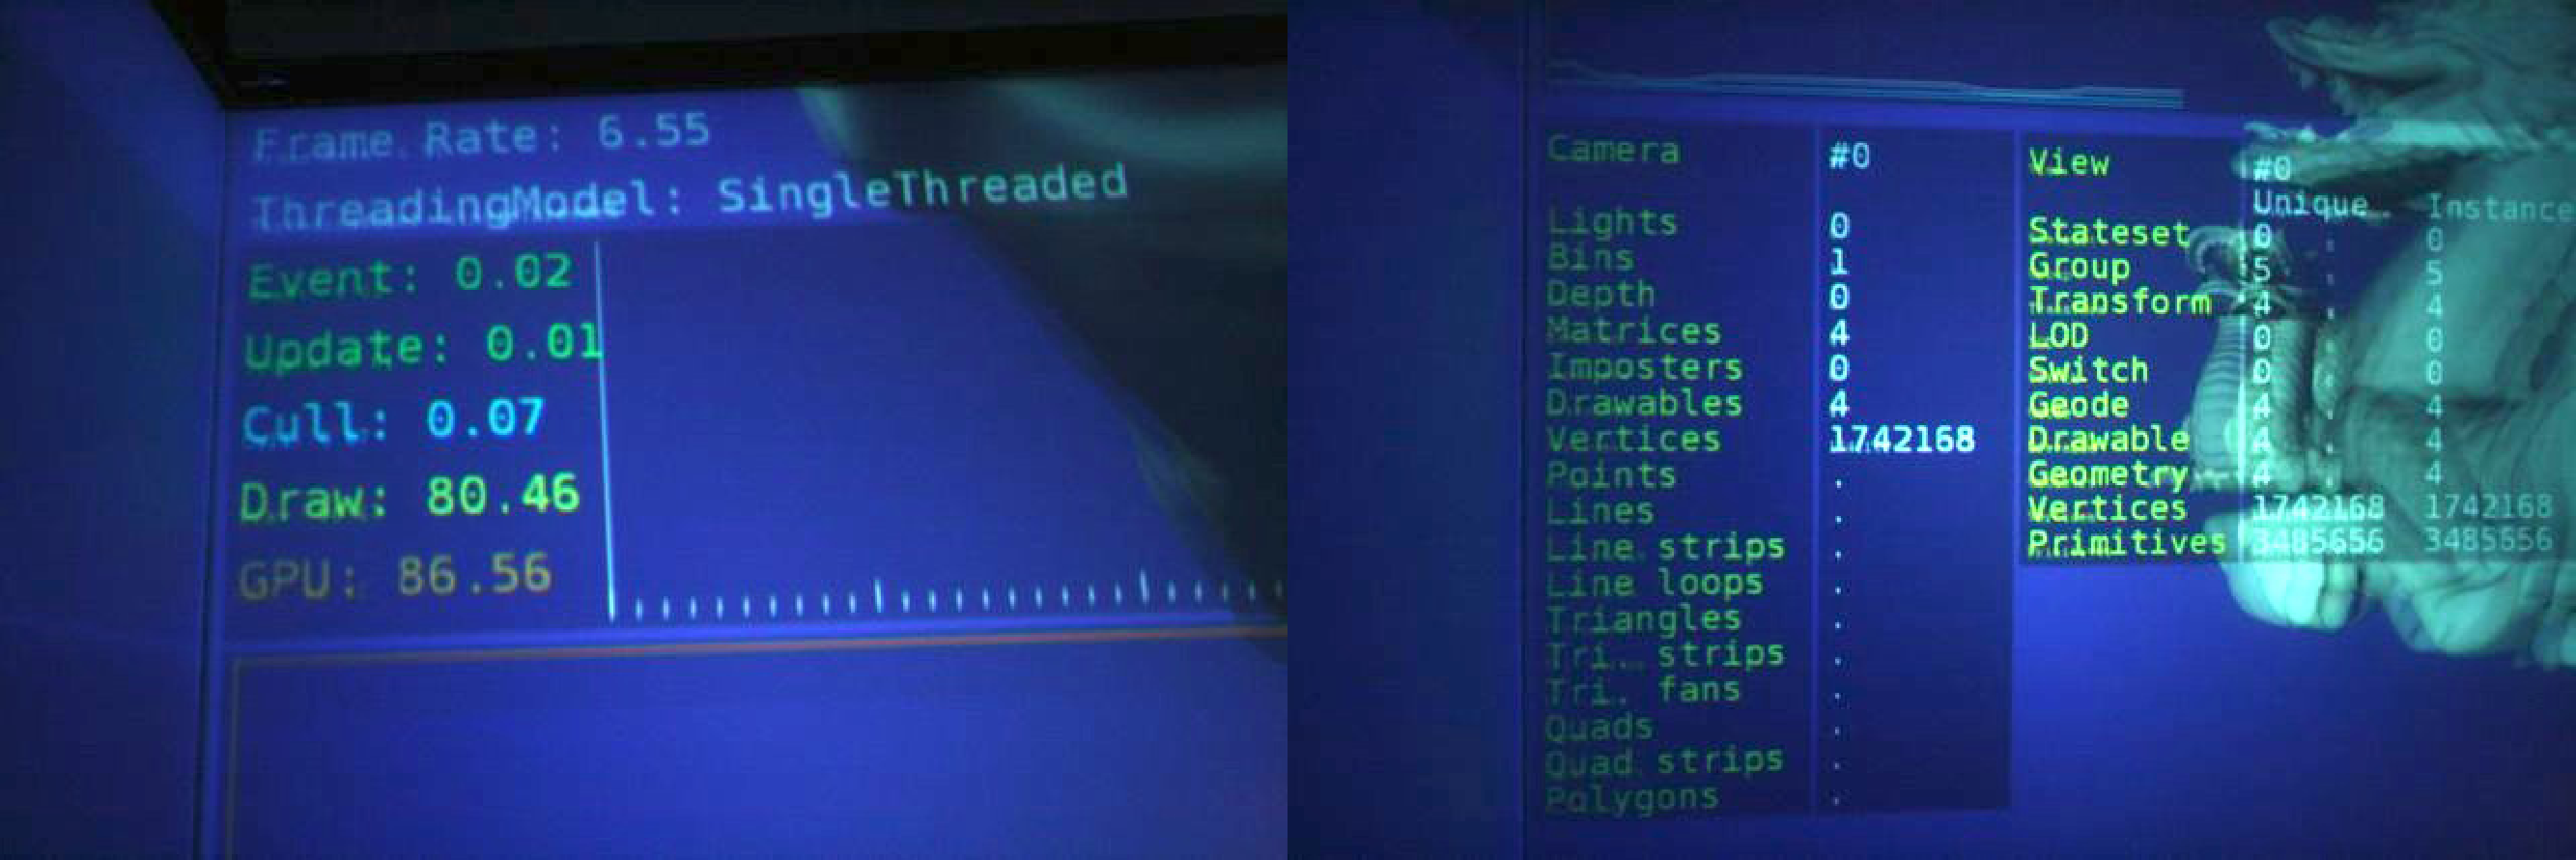
\includegraphics[width=0.9\textwidth]{../figures/fotos/osgStats}
	\caption{OSG statistics}
	\label{fig:osg_stats}
\end{figure}

\subsection{Test Systems}
\begin{table}[H]
	\centering
	\begin{tabular}{|p{0.2\textwidth}|p{0.35\textwidth}|p{0.35\textwidth}|}
			\hline \bfseries Equalizer configuration & 1 node, 8 pipes & 5 nodes, 1pipe each \\
			\hline \bfseries CPU & Intel Quadcore Q9550 @2.8GHz & 2x Intel P4 @3.2GHz \\
			\hline \bfseries Memory & 8GB & 2GB \\
			\hline \bfseries GPU & 4x NVIDIA Quadro FX 1700 & NVIDIA Quadro 3400 \\
			\hline \bfseries Network & \quad\quad- & 1GBit dedicated network \\
			\hline \bfseries OS & \multicolumn{2}{c|}{(X)Ubuntu 8.10} \\
			\hline \bfseries OSG & \multicolumn{2}{c|}{OpenSceneGraph-2.8.1}\\
			\hline \bfseries Equalizer & \multicolumn{2}{c|}{Equalizer-0.6-rc1}\\
			\hline \bfseries Remarks & 1 client with 4 \gls{gpu}s with 2 channels each = 8 Equalizer pipes  & 5 rendering clients with 1 \gls{gpu} and 1 channel each = 5 Equalizer nodes with 1 pipe and 1 channel each \\
			\hline
		\end{tabular}
	\caption{Hardware Setup of Test Environment}
	\label{tab:theUsedTestSystems}
\end{table}

\section{Test Conclusion}

\subsection{OSG Tests}
Most of the tested \gls{osg} scenes rendered properly and produced correct images. With the proper Equalizer configuration the stereoscopic immersion was satisfying and worked out of the box. Moreover, all the tested animated scene graphs worked correctly and even dynamic scenes have been rendered fully synchronously. On rendering clients with multiple \gls{gpu}s and one instance of the running \gls{crf} application, it is very important to implemented the \gls{osg} scene properly (see \nameref{sec:crfLimitations}) to avoid memory abuse.

\subsection{Stress Test}
The most interesting output for our measurements was the \gls{fps}. As mentioned before, we tested two different Equalizer setups. One with a single node, using four graphics cards. The other, a distributed setup with six rendering clients and one server. On the latter, we achieved a more or less constant framerate of 100 \gls{fps} with a model of 1'100'000 triangles. This was about what we expected.

Figure \ref{fig:eq_stats} shows the output of Equalizer measured with the multi-node setup. Equalizer orients itself on the slowest rendering client. The green at the bottom of the statistics represents client number six of the setup. It is the slowest client, meaning, it needs the most time to render a single frame. The five other clients listed above need about 1/5 of the time to render a frame.

\begin{figure}[H]
	\centering
	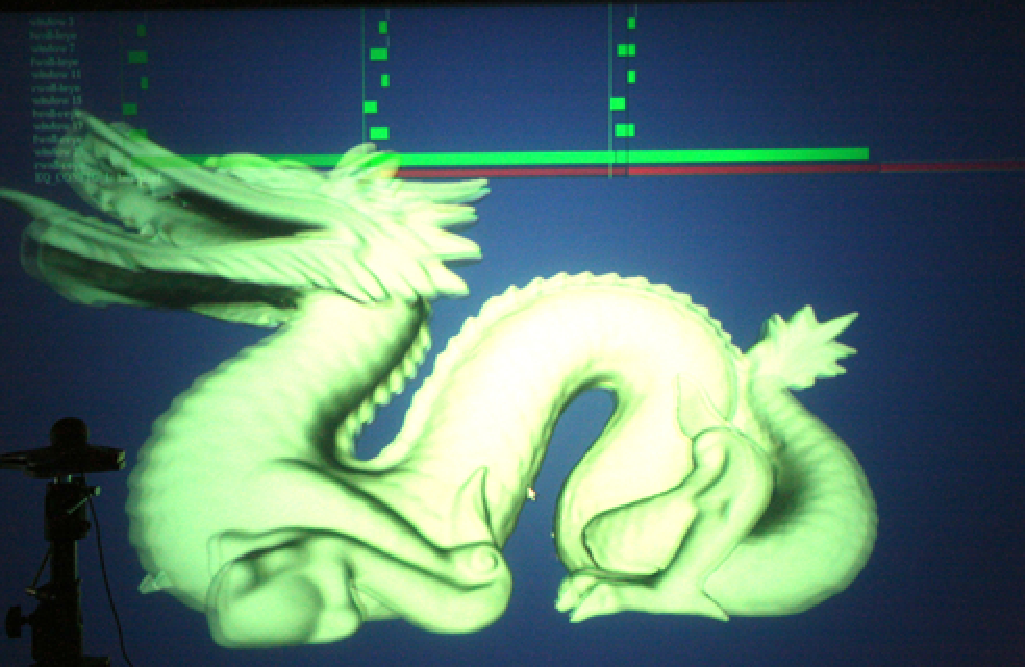
\includegraphics[width=0.5\textwidth]{../figures/fotos/eqStats}
	\caption{Equalizer statistics}
	\label{fig:eq_stats}
\end{figure}
	
The second approach with one computer was less satisfying. With this setup we reached a maximum of 20 \gls{fps}. Conspicuously, the frame rate decreases linearly with each model, even though, they appear on separate walls and should therefore be rendered in different pipes. This behaviour leads to the conclusion that the entire scene graph is rendered on each graphics card. Concerning this issue, we wrote on the Equalizer mailing list. Stefan Eilemann, the founder and developer of Equalizer pointed out that this might be a problem of the NVIDIA graphics driver which could be solved with a later driver release. Other possible reasons he pointed out were:

\begin{itemize}
	\item CPU/Memory contention
	\item Serialisation of the draw calls
	\item Bad multi-threading driver support
	\item Lock contention in \gls{osg} render traversal.
\end{itemize}

The last reason seemed unlikely since the \gls{osg} community never reported similar problems and the eVolve volume rendering demo, shipped with Equalizer, produces bad results too.
